\begin{figure}[H]
  \centering
  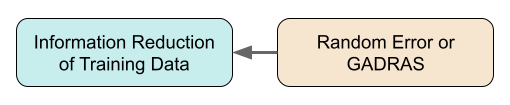
\includegraphics[width=0.7\linewidth]{./chapters/exp1/methodology2.png}
  \caption{Second portion of the flowchart from Figure \ref{fig:method} being 
           described in this section.}
\end{figure}

The overall goal of this project is to determine how much information to what
quality is needed to train an \gls{ML} model that can provide \gls{SNF}
attribution by correctly predicting the reactor type, burnup, \gls{U235}
enrichment, and time since irradiation.  In this section, the information
quality is treated as the information reduction (i.e., increasing error) of
nuclide masses in the training database. 

The training database for the first experiment is meant to be a proof of
principle with the developed methodology, and mimic a scenario where there is
"perfect knowledge" of a set of nuclides of interest. It is still interesting,
however, to probe how the statistical models perform under increasing error in
the nuclide measurements. Therefore error and uncertainty were injected into
the nuclide mass measurements in the training database for the machine learning
algorithms and \gls{MLL} calculations, respectively. 

\noindent \textbf{Machine Learning Algorithms} : For the \textit{k}-nearest
neighbor and decision tree algorithms, a uniform error is applied randomly to
each nuclide mass as follows.  For a maximum error $E_{max}$ between the values
of $0.0 < E_{max} < 0.2$, each nuclide mass is peturbed by a random fraction in
the range: $[1-E_{max},1+E_{max}]$.  Therefore the $0\%$ error case represents
full knowledge of nuclide masses, and that knowledge slowly decreases up to
$20\%$. 

\noindent \textbf{Maximum Likelihood Calculations} : For the \gls{MLL}
calculations, a uniform uncertainty was introduced to each nuclide mass.  Thus,
each nuclide is given an uncertainty of $5\%$, $10\%$, $15\%$, and $20\%$
via:
\begin{equation}
  \label{eq:mllunc}
  \sigma_{Log L}^2 = \sum_j \left( 
                            \frac{r_{j,test} - r_{j,sim}}{\sigma_{j,sim}^2}
                            \right)^2 
                            (\sigma_{j,sim}^2 + \sigma_{j,test}^2)
\end{equation}
where $r_{j,sim}$ and $r_{j,test}$ are the nuclide measurements for the
simulated/training set samples and the test samples, respectively, and
$\sigma_{j,sim}$ and $\sigma_{j,test}$ are their respective standard
deviations calculated from the four uncertainty levels listed above.

